    Herein the term Artificially Intelligent Agent (AIA) will be used in order to encompass a broad range of technologies that can be considered `autonomous'.
    An AIA is defined here as an agent that acts on an internally or externally generated goal, and possesses, to some extent, at least one of the capabilities shown in Fig.~\ref{fig:AIcapabilities} ~\cite{Russell2010-wv,Nilsson2009-rp,Luger2008-vf}. 
    While the term AIA can describe anything from a simple assembly line robot (which only possesses a single capability from Figure~\ref{fig:AIcapabilities}) to the fabled HAL 9000 (who presumably possesses all of the AIA capabilities), this definition underscores the idea that many assurances that exist for one set of (perhaps less capable) AIAs can be adapted and generalized for use in other AIAs.
    In other words, this definition sets a scope for the bodies of research that are likely to have investigated assurances and assurance principles, which can be extended to any `intelligent' computing system. 
    The range of AIA capabilities also helps establish what kinds of assurances might be needed in future systems. 
    For example, assurances for an AIA that only carry out planning tasks will probably differ in design or implementation from assurances for an AIA that only carry out perception tasks. 
    
    It should be noted that an AIA is assumed to operate with a degree of autonomy that is \emph{delegated} by a user. That is, an AIA is self-directed and self-sufficient in its task to the extent that the user's `intent frame' (desired goals, plans, constraints, stipulations and/or value statements) can be met by the AIA, regardless of how it actually accomplishes this. %or what intermediate decisions it needs to make to achieve these ends consistently. 
    Following \citet{Miller2014-av}, this view of autonomy as a delegation relationship refines the need for `transparent AIAs' by avoiding a contradiction of purpose that stems from an otherwise naive interpretation. From a naive standpoint, one could argue that if AIAs are developed primarily to alleviate the burden of complex reasoning and other undesirable workloads by removing users from the task at hand entirely, then this purpose is undercut by exposure and explanation of sophisticated AIA inner workings to the user. 
    However, if AIAs are subordinates that are delegated tasks by users (who must still act as supervisors), the meaning of `transparency' shifts away from concern over how exactly an AIA accomplishes a task, towards concern over whether or not an AIA can execute the task as per the user's intent frame. 
    This delegation-based view naturally sets up the question of user trust in AIAs. 

	\begin{figure}[t!]%[thbp]
    	\centering
     	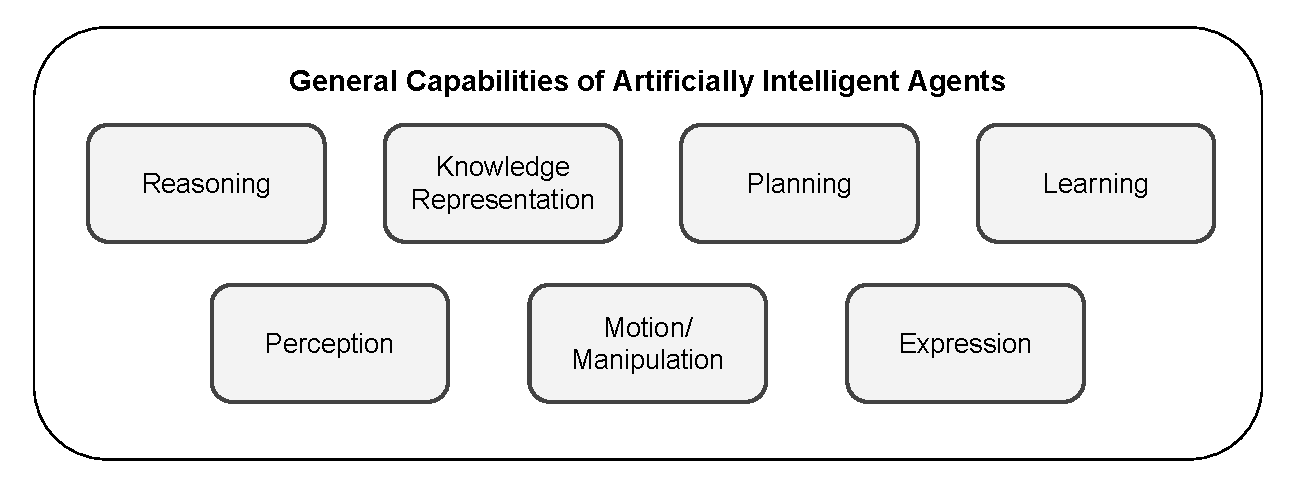
\includegraphics[width=0.55\textwidth]{Figures/AI_capabilities}
    	\caption{Set of possible AIA capabilities.}
        \label{fig:AIcapabilities}
    \end{figure}
